%\documentclass[12pt,preprint]{aastex}
\documentclass[iop]{emulateapj}
\usepackage{natbib,amsmath,graphicx,longtable,amssymb,latexsym,epsf}
\begin{document}

\title{Quasars Probing Quasars IX. Probing the Circumgalactic Flows of Quasars [v1.1]}

\author{Marie Wingyee Lau\altaffilmark{1}, J. Xavier Prochaska\altaffilmark{1}, 
Joseph F. Hennawi\altaffilmark{2}
}
\altaffiltext{1}{Department of Astronomy and Astrophysics, UCO/Lick Observatory, University of 
California, 1156 High Street, Santa Cruz, CA 95064}
\altaffiltext{2}{Max-Planck-Institut f\"ur Astronomie, K\"onigstuhl 17, D-69115 Heidelberg, 
Germany} 

\begin{abstract}
Blah
\end{abstract}


\keywords{glaxies: clusters: intracluster medium -- galaxies: formation -- galaxies: halos -- 
intergalactic medium -- quasars: absorption lines -- quasars: general}

\section{Introduction}

%\begin{itemize}
%\item Flows
%\item Mass (Kaiser, Schaye)
%\item Directionality/symmetry
%\item Break the symmetry
%\end{itemize}

%Take words from my summary of SomervilleDave15. 

The formation and evolution of stars are dictated
by the flow of gas and metals/dust.  [This transport
varies directly with the stellar stage
and a lesser extent stellar mass.]
The accretion onto a protostellar  core eventually
initiates nuclear fusion.  The main sequence is characterized
by gentler stellar winds, with the most massive
stars shedding a cumulative mass of XX\%.
Stellar deaths, meanwhile, are frequently accompanied by terrific
mass loss, occasionally punctuated by a highly energetic,
supernova phase.

By analogy, galaxy formation and evolution are driven by the
flows into/out of their interstellar medium.
In contrast to most stars, however, current theories
predict (even demand) that the star-forming galaxies
maintin these flows. [add]

Akin to stars, direct observations of galactic flows are
difficult to acquire.  Even detecting the gas is challenging:
the gas mass is either too small or the gas density too low
for the [detection] of line-emission (e.g. 21cm, lya,
or H$\alpha$ from Hydrogen).  Resolving the kinematics
and establish the mass-flux represent a far greater challenge.
These challenges are accentuated for distant, young galaxies
where flows are predicted to prevail \citep{keres,fumagalli}.
Therefore, with rare exceptions \citep[e.g.][]{slug,jackpot},
the community has relied on absorption-line spectroscopy
to detect and characterize the gas surrounding galaxies
\citep[e.g.][]{bergeron,steidel10,pro11,tumlinson13}.
With this experiment, researcher have had recent success
in characterizing the large-scale flows around star-forming
galaxies to reveal a net inflow \cite{rakic13} and
provide unique constraints on the mass of the underlying
potential well \cite{rakic14}.

A significant limitation of standard absorption-line
analysis, especially regarding sutyding galactic flows,
is the inherent symmetry of the experiment.
Because one generally lacks any constraint on the distance
of the gas along the sightline,
postive or negative velocities with respect to the
galaxy may be interpreted as gas flowing either towards
or away from the system.
So-called `down-the-barrel' observations break this
symmetry, and have generally provided evidence for flows
away from galaxies \citep{rupke,martin,weiner,rubin}.
However, these data are frequently at low spectral resolution
which limits one's sensitivity to inflowing gas.

In this paper, we examine the flows of gas in the environments
of massive galaxies hosting quasars.  Our approach leverages
a large dataset of quasar pairs \citep{hennawi}
to use the standard technique of absorption-line spectroscopy
with background quasars. [word]
These quasar pairs have angular
separations that correspond to less than 300\,kpc physical
separation at the f/g quasar redshift.
Our previous publications from these quasar pairs
have established that these galaxies are surrounded
by a massive, cool, and enriched circumgalactic medium
\citep{QPQ1,QPQ5,QPQ6,QPQ7}.
We have collected a sample of ntot~spectra passing within
300\,kpc from a f/g quasar with a precisely measured
redshift.  Our primary scientific interests are twofold:
(i) search for signatures of galactic-scale outflows from the
central galaxy, presumably driven by recent star-formation
and/or AGN feedback;
(ii) characterize the dynamics of galactic flows around these
massive system.  We further descrbie an aspect of this
experiment that offers a unique opportunity to study galactic
flows. [detail??]

Throughout this manuscript we adopt a $\Lambda$CDM cosmology with $\Omega_M=0.26, \Omega_\Lambda
=0.74$, and $H_0=70\,{\rm km\,s^{-1}\,Mpc^{-1}}$. All distances are proper unless otherwise 
stated. 
%When referring to comoving distances we include explicitly an $h^{-1}$ term and 
%follow modern convention of scaling to a Hubble constant of $70\,{\rm km\,s^{-1}\,Mpc^{-1}}$. All 
%equivalent width measurements are presented in the rest-frame, unless otherwise specified. 

\section{The Experiment}
\label{sec:data}

From our QPQ survey\footnote{http://www.qpqsurvey.org} (QPQ1), we have analyzed 195~systems 
that pass within 300\,kpc physical from a foreground quasar with $z > 1.6$. We restrict the sample 
to foreground quasars with redshift measured from \ion{Mg}{2}, [\ion{O}{3}], H$\alpha$, or 
H$\beta$ emission, giving a precision of $400\,{\rm km\,s^{-1}}$ or lower. [\ion{O}{3}] has the 
smallest dispersion of $44\,{\rm km\,s^{-1}}$ about the systemic redshift, and we analyze the 
sub-sample with [\ion{O}{3}] redshifts separately. The [\ion{O}{3}] line has an average blueshift 
of $27\,{\rm km\,s^{-1}}$ about the systemic redshift, which has been added when we compute the 
redshift of the line. Systemic redshifts measured from \ion{Mg}{2} have a precision of 
$272\,{\rm km\,s^{-1}}$, and we have taken into account the median redshift of 
$97\,{\rm km\,s^{-1}}$ of \ion{Mg}{2} from [\ion{O}{3}] \citep{Richards+02}. In QPQ8 we have 
quantified the precision of H$\alpha$ and H$\beta$ to be 
$300\,{\rm km\,s^{-1}}$ and $392\,{\rm km\,s^{-1}}$ respectively. 
\citep{hewittwild}.
We include only those spectra with S/N~$> XX$\AA\ at the
observed wavelengths of lya, \ion{C}{2}~1334, or 
\ion{C}{4}~1548 transitions.  Of the ntot~sightlines, 
nhigh\ have spectral resolution ~$> 5,000$ from echellette
or echelle observations (QPQ8).  This high-dispersion 
sample is analyzed [separately] throughout the paper.
Figure~\ref{fig:exp} summarizes the experimental design.
Refer to previous QPQ
publications for details on data reduction
and continuum normalzaton (QPQ6, QPQ7, QPQ8).

%%%%%%%%%%%%%%%%%%%%%%%%%%%%%%%%%%%%%%%%%%%%%%%%%%%%%%%%%%%%
%%%%%%%%%%%%%%%%%%%%%%%%%%%%%%%%%%%%%%%%%%%%%%%%%%%%%%%%%%%%
\section{Analysis}
\label{sec:analysis}

In QPQ8, we measured the velocity widths of the \ion{C}{2}~1334
and \ion{C}{4}~1548 transitions finding that the CGM
frequently exhibits large flows:
median DV{1334},DV{1548} = $XX,XX kms$ with and
RMS DRMS{1334},DRMS{1548} = $XX, XX kms$ from
a sample of ncii\ and nciv\ systems.
These velocity fields exceed all previous measurements from
galaxies and/or absorption systems at any epoch.  For
Figure~\ref{fig:stack}, we present these absorption lines
and \ion{H}{1}~lya, also including lower-dispersion 
sightlines meeting the selection criteria.

To assess the `average' absorption of these transitions,
we have combined the data with a novel technique.
We have fitted the combined dataset using a cubic b-spline
with knots at every 100\,kms.  We weighted each data
point by the velocity width of the pixel to insure that 
each sightline makes an equal contribution to the stack.
These b-spline profiles are presented in the figure
and a trivial integration gives the reported equivalent
widths.
[consider down-weighting systems with $<3\sigma$ EW]
[Comnent on EW from 'standard' technique]

Two results are evident from the figure:
 (i) the data exhibit excess absorptoin at 
 $mdv \approx 0 kms$;
 (ii) the absorption is skewed towards positive velocities
 $mdv > 0 mkms$.
We measure absorption-weigthed ($1-f$) centroids
of $mdv = XX-XX mkms$ for these transitions
(Table~\ref{tab:summ}).
This suggests an asymmetry that contradicts the [standard]
expectation.  

Given the small sample size, one must 
scrutinize the statistical significance of the measured offset.
Indeed, a small offset $mdv < 10 kms$ may be expected
even with large samples.  To assess the statistical significance,
we have perfomed a boostrap analysis by randomly resampling
from the full sample. [DISCUSS]

[Discuss systematics here??]

%%%%%%%%%%%%%%%%%%%%%%%%%%%%%%%%%%%%%%%%%%%%%%%%%%%%%%%%%%%%
%%%%%%%%%%%%%%%%%%%%%%%%%%%%%%%%%%%%%%%%%%%%%%%%%%%%%%%%%%%%
\section{Discussion}
\label{sec:discussion}

[Add a cartoon fig with cone]
[Is it really obvious that this works??]


%%%%%%%%%%%%%%%%
\acknowledgements

JXP and ML acknowledge support from the National
Science Foundation (NSF) grant AST-1010004 and AST-XX. 
JXP thanks the Alexander
von Humboldt foundation for a visitor fellowship to the MPIA where
part of this work was performed, as well as the staff at MPIA for
their hospitality during his visits.
JFH acknowledges generous support from the Alexander von Humboldt
foundation in the context of the Sofja Kovalevskaja Award. The
Humboldt foundation is funded by the German Federal Ministry for
Education and Research.  

%Much of the data presented herein were obtained at the W.M. Keck
%Observatory, which is operated as a scientific partnership among the
%California Institute of Technology, the University of California, and
%the National Aeronautics and Space Administration. The Observatory was
%made possible by the generous financial support of the W.M. Keck
%Foundation.  Some of the Keck data were obtained through the NSF
%Telescope System Instrumentation Program (TSIP), supported by AURA
%through the NSF under AURA Cooperative Agreement AST 01-32798 as
%amended.
%
%Some of the data herein were obtained at the Gemini Observatory, which
%is operated by the Association of Universities for Research in
%%Astronomy, Inc., under a cooperative agreement with the NSF on behalf
%of the Gemini partnership: the NSF (United
%States), the Science and Technology Facilities Council (United
%Kingdom), the National Research Council (Canada), CONICYT (Chile), the
%Australian Research Council (Australia), Minist\'{e}rio da
%Ci\^{e}ncia, Tecnologia e Inova\c{c}\~{a}o (Brazil) and Ministerio de
%Ciencia, Tecnolog\'{i}a e Innovaci\'{o}n Productiva (Argentina). 
%
%The authors wish to recognize and acknowledge the very
%significant cultural role and reverence that the summit of Mauna Kea
%has always had within the indigenous Hawaiian community. We are most
%fortunate to have the opportunity to conduct observations from this
%mountain.
%Acknowledge TK Chan. CP Choi.


\bibliographystyle{/u/xavier/paper/Bibli/apj}
\bibliography{/u/xavier/paper/Bibli/allrefs}

%%%%%%%%%%%%%%%%%%%%%%%%%%%%%%%%%%%
%\input{../Tables/tab_sub_qpq7_spectra.tex}
\begin{deluxetable*}{lccc}
\tablewidth{0pc}
\tablecaption{Summary of Experimental Design and Analysis for the Full QPQ9 Sample
\label{tab:summary}}
\tabletypesize{\small}
\tablehead{\colhead{Measure} & \colhead{\ion{C}{2}\,1334} & \colhead{\ion{C}{4}\,1548} 
& \colhead{\ion{Mg}{2}\,2796}} 
\startdata 
Number of pairs & 34 & 92 & 26 \\ 
Median $z_{\rm fg}$ & 2.03 & 1.94 & 1.88 \\ 
Median $R_\perp$ (kpc) & 180 & 189 & 150 \\ 
Centroid of mean-stacked spectrum (${\rm km\,s^{-1}}$) & $+170\pm121$ & $+53\pm105$ & $+161\pm108$ \\
1$\sigma$ dispersion of mean stack (${\rm km\,s^{-1}}$) & 388 & 363 & 340 \\
Centroid of median-stacked spectrum (${\rm km\,s^{-1}}$) & $+16\pm106$ & $+181\pm106$ & $-12\pm162$ \\
1$\sigma$ dispersion of median stack (${\rm km\,s^{-1}}$) & 313 & 320 & 207 \\
\enddata 
\end{deluxetable*} 

%\input{Tables/tab_summ_Hab.tex}
%\input{tab1_sub.tex}


%%%%%%%%%%%%%%%%%%%%%%%%%%%%%%%%%%%%%%%%%%%%%%%%%%%%%%%%%
%%%%%%%%%%%%%%%%%%%%%%%%%%%%%%%%%%%%%%%%%%%%%%%%%%%%%%%%%
%%%%%%%%%%%%%%%%%%%%%%%%%%%%%%%%%%%%%%%%%%%%%%%%%%%%%%%%%

\clearpage

\begin{figure}
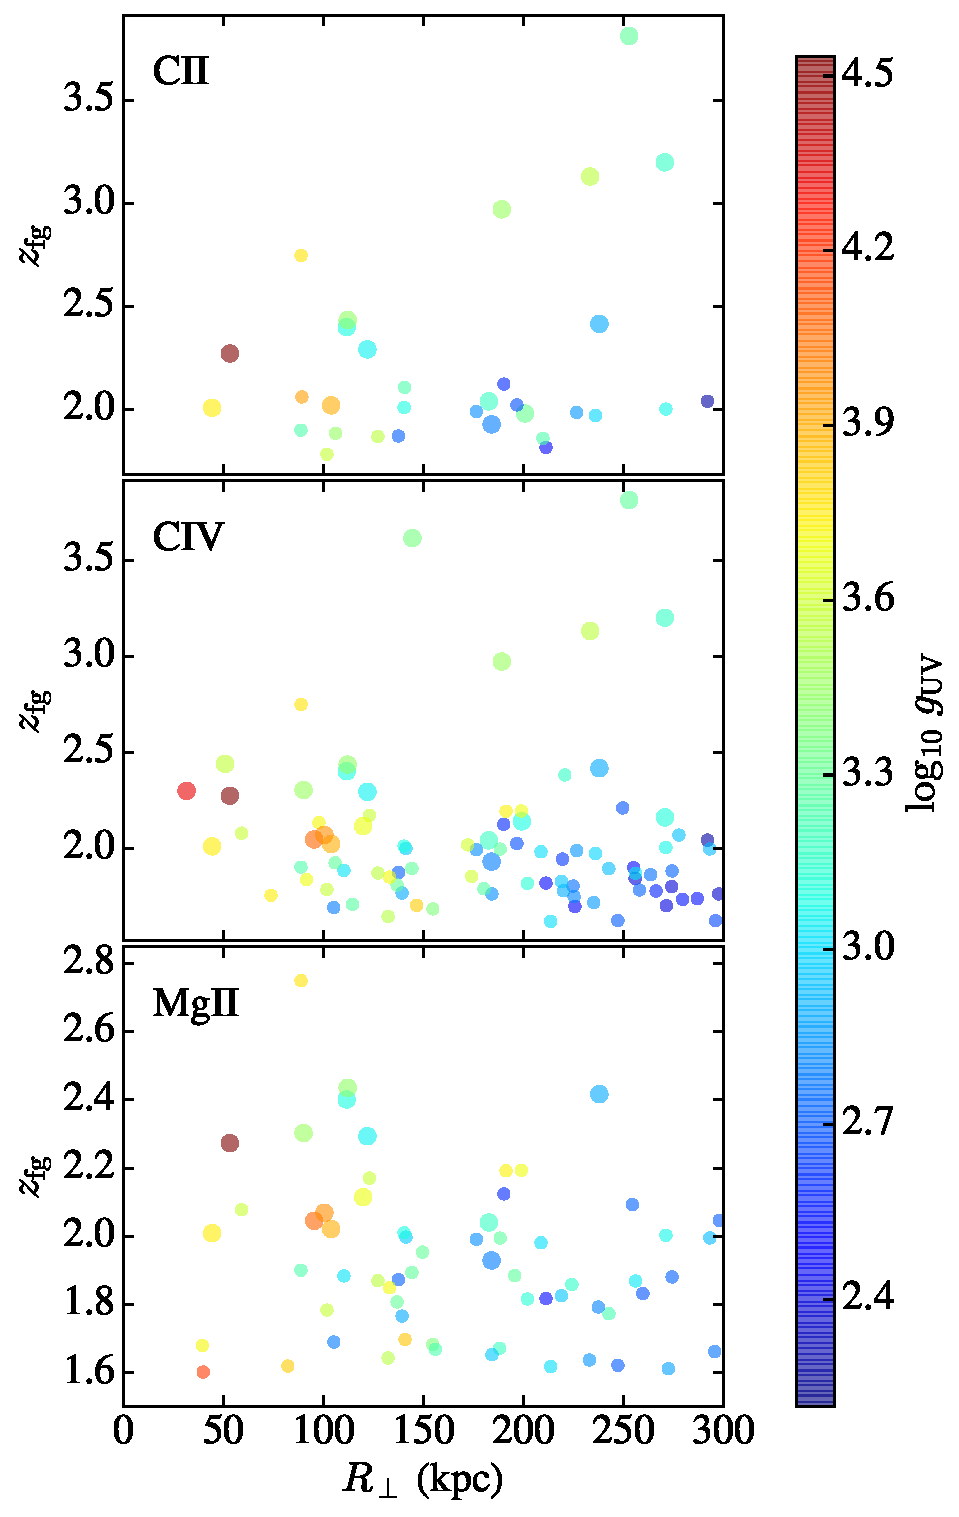
\includegraphics[width=5in]{Figures/fig_experiment.pdf}
%\includegraphics[width=5in,angle=90]{../Figuref1.eps}
\caption{Experimental design
}
\label{fig:exp}
\end{figure}

\begin{figure}
%\includegraphics[width=5in]{Figures/fig_simple_stack.pdf}
%\includegraphics[width=5in,angle=90]{f2.eps}
\caption{Simple stack
}
\label{fig:stack}
\end{figure}

\end{document}
